%% ===========================================================================
%% Lab 8 — Capstone Research Proposal (IEEE two-column conference format)
%% "Benchmarking Minimax Search, Imitation of Human Play, Self-Play Reinforcement
%%  Learning, and Monte Carlo Tree Search over Policy-Value Networks to Identify
%%  the Strongest Paradigm in a Multi-Agent Xiangqi League"
%%
%% Compile:  xelatex main  ->  bibtex main  ->  xelatex main  ->  xelatex main
%% (or: latexmk -xelatex main  /  tectonic main.tex)  [fontspec needs XeLaTeX]
%% Target: 4 pages maximum, including references.
%% ===========================================================================
\documentclass[conference]{IEEEtran}
\IEEEoverridecommandlockouts

\usepackage{fontspec}
\setmainfont{texgyretermes}[
  Extension = .otf,
  UprightFont = *-regular,
  BoldFont = *-bold,
  ItalicFont = *-italic,
  BoldItalicFont = *-bolditalic ]
% CJK font (Noto Serif SC) for the author's Chinese name and Chinese terms
\newfontfamily\cjkfont{NotoSerifSC}[Path=./, Extension=.ttf]
\newcommand{\zh}[1]{{\cjkfont #1}}
\usepackage{cite}
\usepackage{amsmath,amssymb}
\usepackage{graphicx}
\usepackage{booktabs}
\usepackage[hidelinks]{hyperref}

\begin{document}

\title{\fontsize{16}{19}\bfseries\selectfont Benchmarking Minimax, Imitation,
Self-Play Reinforcement Learning, and Monte Carlo Tree Search in a Multi-Agent
Xiangqi (\zh{象棋}) League}

\author{%
\IEEEauthorblockN{Alma Nurul Salma (\zh{诺艾玛})}
\IEEEauthorblockA{Nanjing Xiaozhuang University (\zh{南京晓庄学院})\\
Student ID: L25020007\\
Email: almanurulsalma@gmail.com}
}

\maketitle

\begin{abstract}
Modern game-playing agents are built from three ideas validated on Go and chess
at cluster scale: imitation of human experts, reinforcement learning by
self-play, and tree search over a learned network. It is unknown which of these
paradigms plays strongest for \emph{Xiangqi} (\zh{象棋}, Chinese Chess), whether
imitation pretraining still helps the subsequent reinforcement learning, and what
factor ultimately bounds playing strength, because no study compares them
head-to-head. Existing Xiangqi
deep-learning work consists of a few single-system papers and provides no
controlled, like-for-like comparison. We propose a controlled, head-to-head
study that places four paradigms---classical alpha--beta search, pure-self-play
Proximal Policy Optimization, imitation-initialised Proximal Policy Optimization,
and AlphaZero-style Monte Carlo Tree Search---on a single shared Xiangqi engine, a
fixed 2086-move action space, one policy--value network, and one Elo scale, so the
paradigm is the only variable. We rank the agents by fitted Elo with 95\%
confidence intervals, quantify the effect of imitation pretraining on the
subsequent reinforcement learning, and run a four-lever ablation (search, epochs,
teacher, network size) to identify the binding constraint. A complete, tested
implementation and preliminary runs over a 9.3M-position training split (113k of
141{,}356 human games, 11.6M positions in all) already exist, making the study a
rigorous formalisation rather than a
speculative build. The expected contributions are a reusable multi-agent
evaluation framework, to our knowledge the first controlled, head-to-head paradigm
comparison for Xiangqi, and reproducibility guidance for self-play
reinforcement learning.
\end{abstract}

\begin{IEEEkeywords}
Xiangqi, Chinese Chess, deep reinforcement learning, Monte Carlo Tree Search,
imitation learning, Proximal Policy Optimization, Elo rating, empirical software
engineering, reproducibility.
\end{IEEEkeywords}

\section{Introduction}
\IEEEPARstart{T}{he} dominant recipe for superhuman board-game play was
established on Go by AlphaGo, which combined supervised (imitation) learning of
expert moves, reinforcement learning by self-play, and Monte Carlo Tree Search
\cite{silver2016}. AlphaGo~Zero removed the human-data stage and learned
\emph{tabula rasa} \cite{silver2017}, and AlphaZero generalised the same
algorithm to chess, shogi, and Go, replacing alpha--beta search with general
Monte Carlo Tree Search \cite{silver2018}. These landmark results share two
properties that limit their guidance for most practitioners: they were obtained
on large tensor-processing clusters, and each reports a single successful pipeline
rather than a controlled comparison of the paradigms it combines.

\textbf{Motivation and problem.} These practical questions---which paradigm plays
strongest, and why---are unanswered, especially for
\emph{Xiangqi} (\zh{象棋}, Chinese Chess)---a culturally major but
academically under-served game with a larger $9\times10$ board, higher branching
than chess, a cannon that captures by jumping a screen, and the unusual rule that
\emph{stalemate is a loss} (Fig.~\ref{fig:board}). The published deep-learning work on Xiangqi is recent
and sparse: an AlphaZero-style player that searches with Monte Carlo Tree Search
\cite{yilmaz2025}, a population method that tackles strategic non-transitivity
\cite{li2023jiangjun}, and a language-model approach trained with policy
optimization \cite{xiangqir1}. Each builds \emph{one} maximally strong system;
none compares the distinct learning paradigms head-to-head---which plays strongest,
whether imitation pretraining helps the reinforcement learning that follows, or
which factor limits strength.

\begin{figure*}[t]
\centering
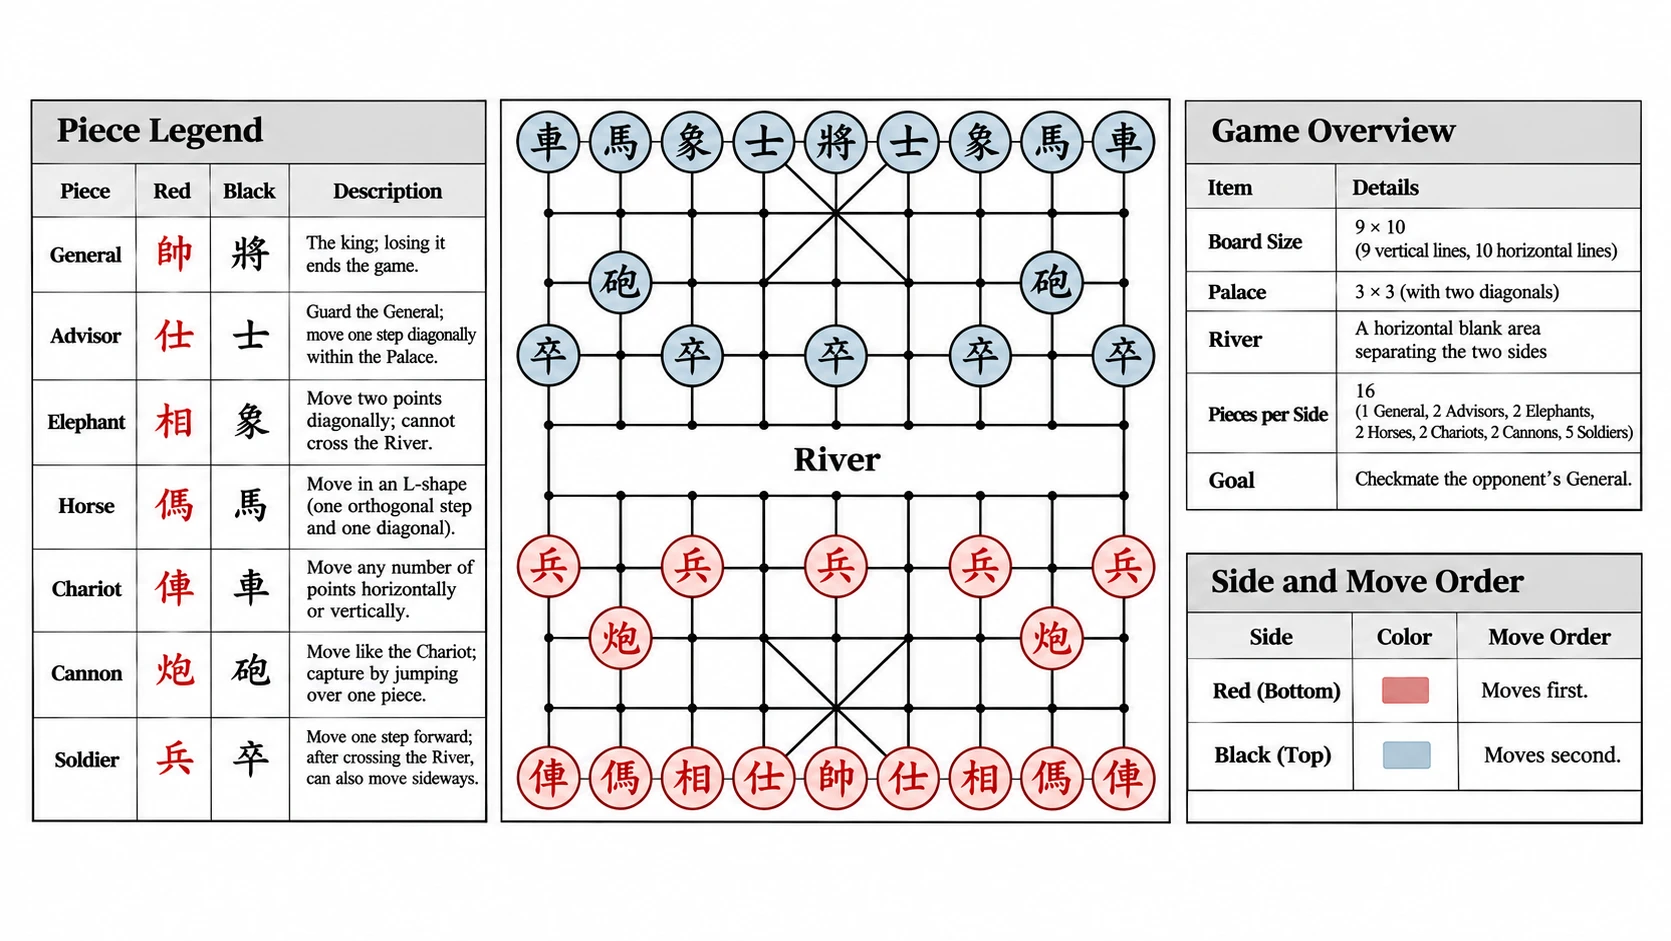
\includegraphics[width=0.48\textwidth]{figures/gfig1_board.png}\hfill
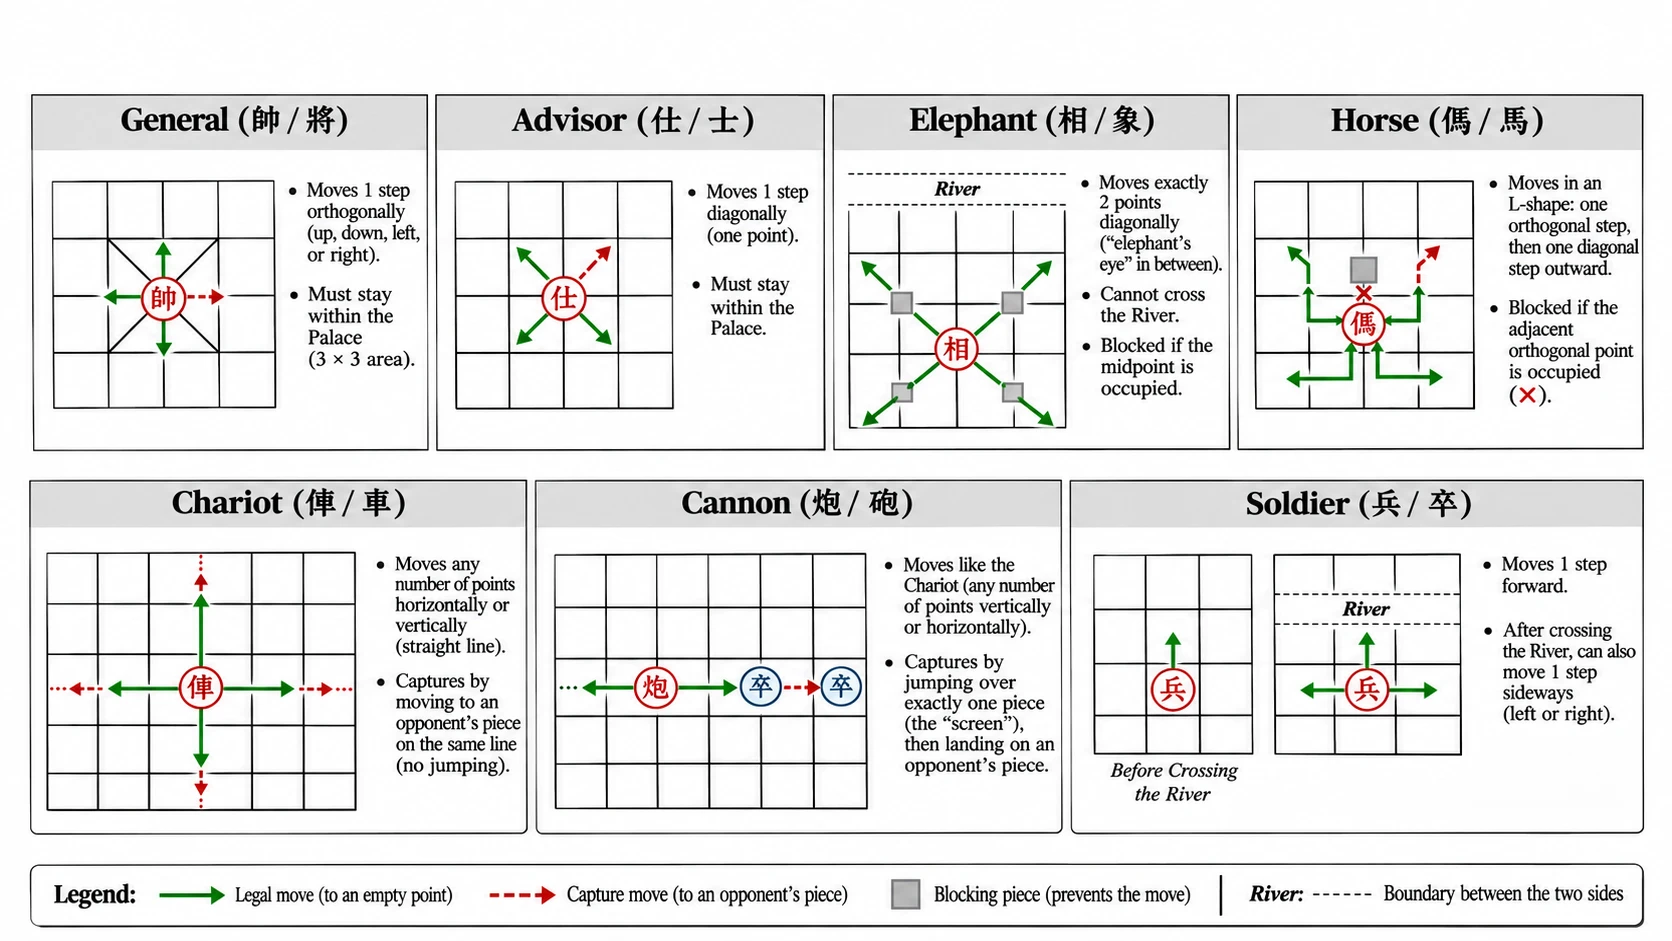
\includegraphics[width=0.48\textwidth]{figures/gfig2_moves.png}
\caption{\emph{Left:} the $9\times10$ Xiangqi (\zh{象棋}) board with its river and
two palaces, the opening position, and the seven piece types (Red moves first).
\emph{Right:} how each piece moves and captures---the cannon's jump-the-screen
capture and the horse's blockable leg give Xiangqi tactics without a chess
analogue, enlarging the branching factor the agents must search.}
\label{fig:board}
\end{figure*}

\textbf{Significance.} Deep reinforcement-learning results are known to be fragile
and hard to reproduce when reported from single runs without variance analysis
\cite{henderson2018}. A controlled, confidence-interval-backed comparison on one
rule engine therefore yields decision-relevant, reproducible evidence that
cluster-scale, single-system papers do not.

\textbf{Research questions.} We pose three questions, each answerable by the
methodology below:
\begin{itemize}
\item \textbf{RQ1 (ranking):} how do the four
paradigms rank in Xiangqi playing strength on a common Elo scale?
\item \textbf{RQ2 (effect of imitation pretraining):} does imitation pretraining
improve the subsequent Proximal Policy Optimization self-play,
or can reinforcement learning fine-tuning \emph{degrade} the imitation policy?
\item \textbf{RQ3 (binding constraint):} which factor---play-time search, model
capacity, training data or teacher, or the learning algorithm---most limits
playing strength at this scale?
\end{itemize}

\textbf{Proposed solution.} We hold the environment, action space, network, and
Elo scale fixed and swap \emph{only} the learning paradigm, so a like-for-like
ranking isolates the effect of the paradigm itself.

\section{Related Work}
\textbf{Deep learning, search, and imitation.} The AlphaGo family established the
two levers we compare---imitation pretraining and search over a learned network
\cite{silver2016,silver2017,silver2018}---with Monte Carlo Tree Search surveyed by
Browne \textit{et al.} \cite{browne2012}, whose selection rules our search agent
builds on; classical Xiangqi engines instead use alpha--beta search with
handcrafted evaluation, the tradition our Minimax baseline represents. A known
limitation of the imitation stage is that an imitator cannot surpass its
demonstrators---the usual justification for the reinforcement-learning stage---but
whether that stage actually helps is untested for Xiangqi, and
our preliminary data suggest it can hurt.

\textbf{Policy gradients and reproducibility.} Proximal Policy Optimization
\cite{schulman2017} is our reinforcement-learning optimizer, chosen for stability;
yet Henderson \textit{et al.} \cite{henderson2018} show policy-gradient results
vary sharply with seeds and implementation, motivating our interval-based
evaluation and a training-stability analysis.

\textbf{Populations and Xiangqi-specific work.} AlphaStar rated a league of
adapting agents on an Elo ladder \cite{vinyals2019}, a framing we adopt for
\emph{heterogeneous} agents. The directly comparable Xiangqi systems each optimise
one pipeline at cluster scale or without cross-paradigm comparison: an
AlphaZero-style player \cite{yilmaz2025}, JiangJun, which combines Monte Carlo Tree
Search with Policy-Space Response Oracles over $>$10{,}000 human games to address
non-transitivity \cite{li2023jiangjun}, and a language-model approach
\cite{xiangqir1}. Table~\ref{tab:gap} summarises the resulting gap.

\begin{table}[t]
\caption{Where prior work leaves the gap this study fills.}
\label{tab:gap}
\centering
\footnotesize
\resizebox{\columnwidth}{!}{%
\begin{tabular}{@{}lccc@{}}
\toprule
Work & Xiangqi & Cross-paradigm & Equal- \\
     &         & comparison     & compute \\
\midrule
AlphaGo family \cite{silver2016,silver2017,silver2018} & no & no & no \\
Monte Carlo Tree Search survey \cite{browne2012} & n/a & n/a & n/a \\
Proximal Policy Optimization \cite{schulman2017} & no  & partial & no \\
Reproducibility \cite{henderson2018}        & no & no & yes \\
AlphaStar \cite{vinyals2019}                & no  & no  & no \\
JiangJun \cite{li2023jiangjun}              & yes & no  & no \\
Yilmaz \textit{et al.} \cite{yilmaz2025}    & yes & no & partial \\
Xiangqi-R1 \cite{xiangqir1}                 & yes & no  & partial \\
\textbf{This study}                         & \textbf{yes} & \textbf{yes} & \textbf{yes} \\
\bottomrule
\end{tabular}}
\end{table}

\textbf{Research gap.} No controlled, head-to-head, Elo-anchored comparison of
classical search, pure Proximal Policy Optimization, imitation-initialised
Proximal Policy Optimization, and AlphaZero-style Monte Carlo Tree Search exists
for Xiangqi; consequently the direction of the
imitation-pretraining effect and the binding constraint on strength are both
unquantified for this game. This is primarily an
\emph{evaluation/methodological} gap, with secondary \emph{performance} and
\emph{application} dimensions.

\section{Proposed Methodology}
\textbf{Design.} A controlled comparative study: the independent variable is the
paradigm (or the one ablated lever); the dependent variable is Elo; everything
else is fixed by a shared stack (Fig.~\ref{fig:arch}), so differences in strength
are attributable to the decision function alone. ``Equal effort'' is
operationalised as a matched number of self-play environment steps per
reinforcement-learning agent, reported beside every result so the comparison is
fair rather than open-ended.

\begin{figure*}[t]
\centering
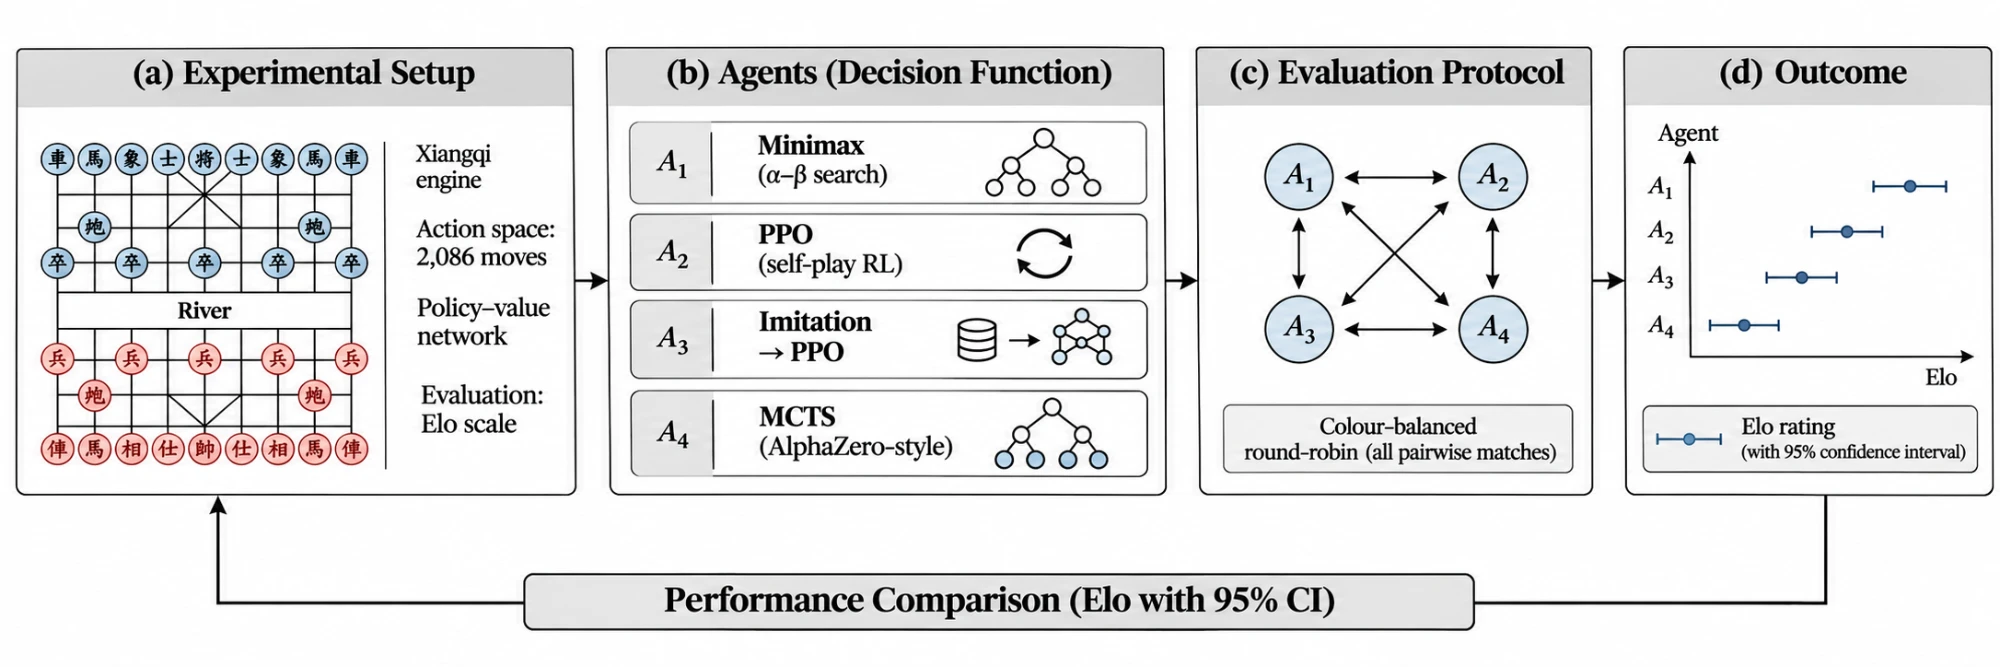
\includegraphics[width=0.80\textwidth]{figures/gfig4_framework.png}
\caption{The controlled apparatus. One shared engine, action space, and
policy--value network feed four interchangeable decision functions---the only
variable---and all agents are rated on a single Elo scale by a colour-balanced
round-robin anchored to Pikafish.}
\label{fig:arch}
\end{figure*}

\textbf{Shared components.} (1) A tested Xiangqi rule engine exposed through a
Gymnasium interface, with a fixed 2086-move action space and legal masking, and a
$14\times10\times9$ side-to-move-relative board encoding. (2) One AlphaZero-style
policy--value network reused by imitation, by Proximal Policy Optimization (as
actor and critic), and by Monte Carlo Tree Search (as priors and leaf value); its
width and depth are configurable for the ablation (Fig.~\ref{fig:tensor}).

\begin{figure}[t]
\centering
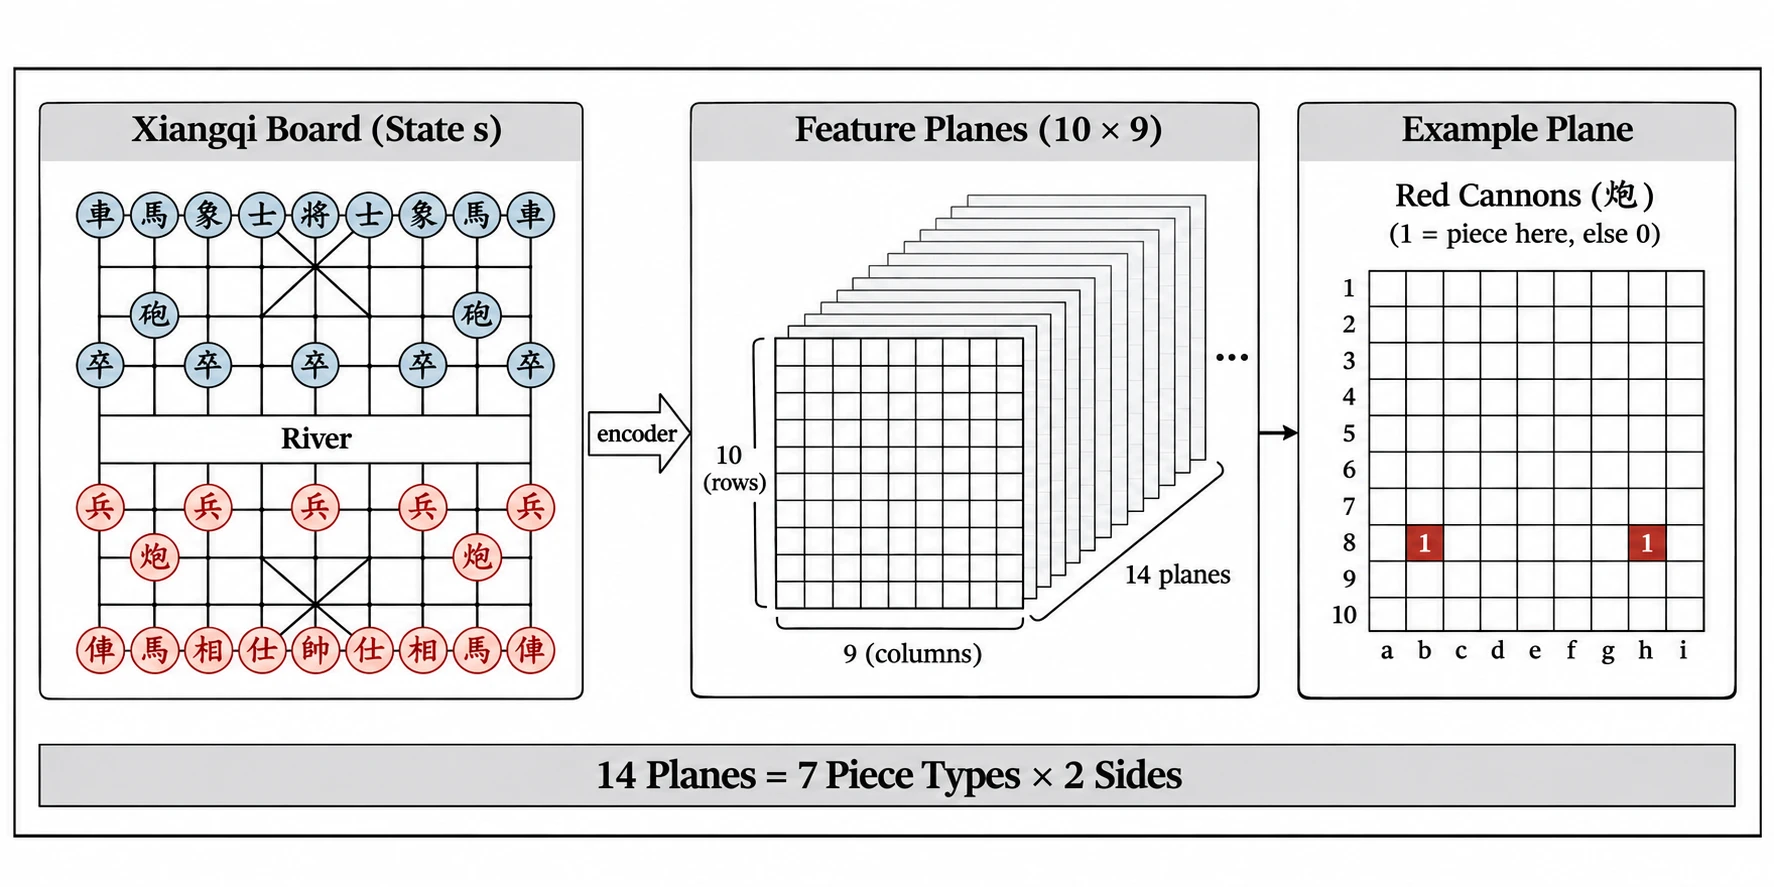
\includegraphics[width=0.85\columnwidth]{figures/gfig3_tensor.png}
\caption{The board is encoded as a $14\times10\times9$ tensor---one $10\times9$
binary plane per piece type and side, from the side-to-move's perspective, shared
by every agent.}
\label{fig:tensor}
\end{figure}

\textbf{The four agents.} \emph{Minimax}: alpha--beta (negamax) search with a
material evaluation. \emph{From-scratch Proximal Policy Optimization}:
action-masked self-play from random initialisation. \emph{Imitation-initialised
Proximal Policy Optimization}: supervised imitation of 113k human games, then
action-masked self-play refinement from that checkpoint. \emph{Monte Carlo Tree
Search agent}: a best-first search that uses the network's priors to guide
selection and its value head to evaluate leaves, choosing moves by visit count. A
random agent is included as a floor.

\textbf{Data.} 141{,}356 legal human games ($\approx$11.6M positions) are split at
the game level into 113k/14k/14k train/validation/test sets, recorded in a
committed manifest for reproducibility; an engine self-play corpus supports the
teacher-distillation lever.

\textbf{Procedure.} Each reinforcement-learning paradigm is trained to a matched
number of self-play steps with periodic checkpointing. \emph{Experiment~1 (RQ1)} runs a
colour-balanced round-robin among all four agents plus the random agent and fits
Elo with 95\% confidence intervals using \eqref{eq:elo} and a head-to-head matrix.
\emph{Experiment~2 (RQ2)} isolates imitation-only, imitation-initialised Proximal
Policy Optimization, and from-scratch Proximal Policy Optimization and reports the
signed Elo differences plus learning proxies (imitation top-1 accuracy;
self-play reward and value traces). \emph{Experiment~3 (RQ3)} varies one lever at
a time---search simulations $\in\{100,200,400,800\}$, imitation epochs, teacher
(human versus engine distillation), and network size ($1.15$M versus $4.85$M
parameters)---each re-entered into the round-robin, reporting each lever's Elo
effect. A stability study compares fragmented, continuous, and
replay-buffer-persisted training.

\textbf{Evaluation metrics.} The expected score of a rating difference is
\begin{equation}
\label{eq:elo}
E_A = \frac{1}{1 + 10^{(R_B - R_A)/400}},
\end{equation}
inverted and fitted over round-robin results to obtain each agent's rating;
confidence intervals follow the delta method. The imitation stage minimises the
policy--value loss $\mathcal{L}_{\mathrm{IL}}{=}\mathrm{CE}(\pi_\theta,
a_{\text{human}}){+}\mathrm{MSE}(v_\theta,z)$, and the search agent selects the
move maximising the prior-weighted PUCT score. Reported metrics are fitted and
absolute Elo (with 95\% confidence interval), head-to-head win rates, the signed
Elo difference between the imitation-only and imitation-initialised agents,
per-lever Elo effects, top-1 move accuracy, value-loss trajectories, and GPU-hour
cost. Differences are called significant only when confidence intervals do not
overlap; non-transitivity is handled by full round-robins and fitted Elo rather
than single matches \cite{li2023jiangjun}. Fixed seeds, the committed manifest,
and per-run configuration, seed, and commit logging address known reproducibility
pitfalls \cite{henderson2018}.

\textbf{Threats to validity.} Relative Elo depends on the pool (mitigated by an
absolute Pikafish anchor and full round-robins); few games per pair widen the
intervals (mitigated by rerunning decisive comparisons with more games); the
shared-stack design keeps the comparison internally valid, since only the
decision function varies.

\section{Expected Results and Contributions}
\textbf{Expected outcomes.} We hypothesise that (H1) the Monte Carlo Tree Search
agent attains the highest Elo; (H2) imitation pretraining raises \emph{starting}
strength but, under the constrained budget, self-play reinforcement learning does
\emph{not} raise the ceiling and may lower it; and (H3) model capacity and
training data---not search depth or the learning algorithm---bind strength.
Preliminary runs on the existing implementation are consistent with all three and
establish feasibility (Fig.~\ref{fig:elo}); these are \emph{preliminary,
confidence-interval-wide} measurements that the proposed study will formalise with
more games and tighter intervals, not final results.

\begin{figure*}[t]
\centering
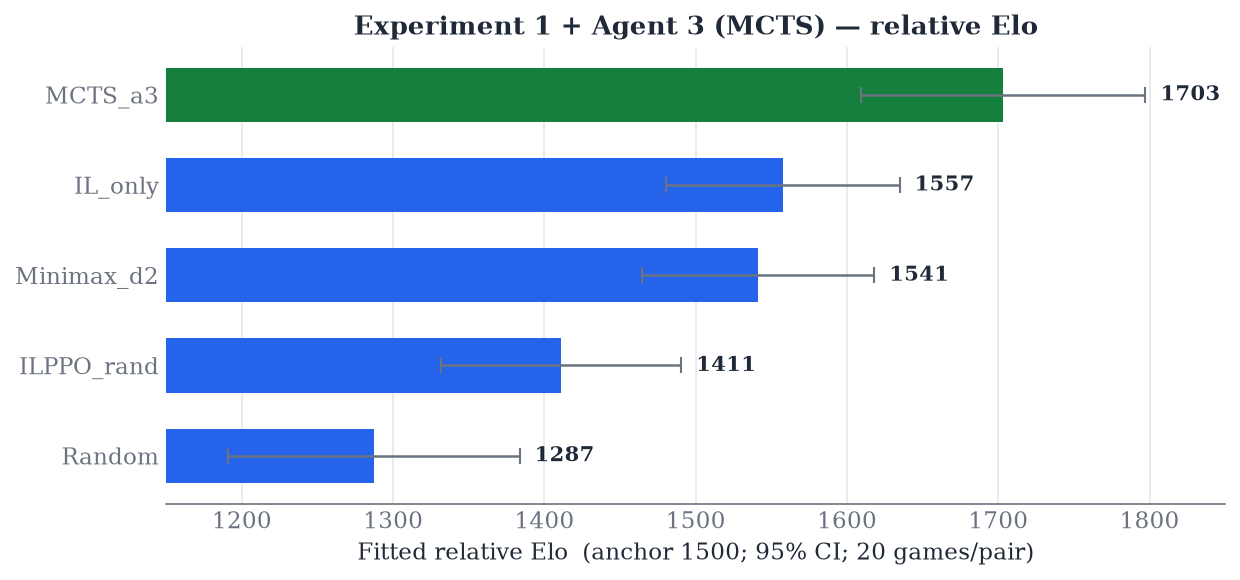
\includegraphics[height=46mm]{figures/elo_bars.png}\hspace{6mm}%
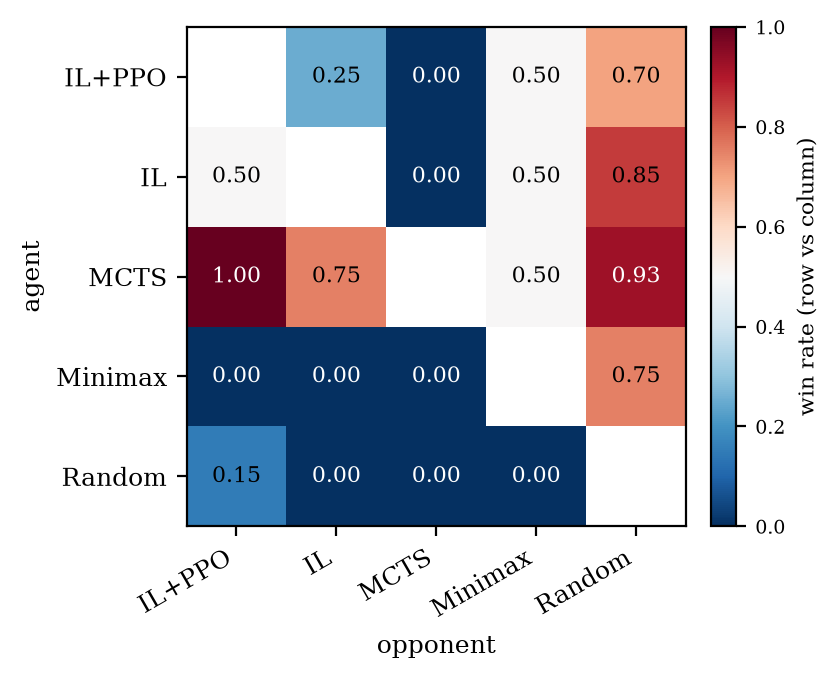
\includegraphics[height=46mm]{figures/headtohead.png}
\caption{Preliminary feasibility measurements. \emph{Left:} fitted relative Elo
(anchor 1500) with 95\% confidence intervals from a round-robin of the four
paradigms plus a random agent; a stabilised rerun reproduced the same top rank
(Monte Carlo Tree Search $\approx$1691). \emph{Right:} head-to-head win rates (row
agent vs.\ column opponent)---the Monte Carlo Tree Search agent dominates its
column and the ladder is largely transitive, with many draws under the 300-ply
cap.}
\label{fig:elo}
\end{figure*}

\textbf{Contributions.} (1) \emph{Technical}: a reusable, single-interface
multi-agent evaluation league for comparing heterogeneous game-playing paradigms
on one rule engine, runnable on a single consumer GPU. (2) \emph{Research}: a
controlled, head-to-head, Elo-anchored comparison of the four paradigms for
Xiangqi, a quantified answer to whether imitation pretraining helps the subsequent
reinforcement learning, and a multi-lever capacity-bottleneck
analysis. (3) \emph{Software engineering}: evidence that training-stability
engineering---replay-buffer continuity and best-checkpoint selection---materially
affects learned-model quality, yielding reproducibility guidance for self-play
reinforcement learning.

\textbf{Timeline.} The apparatus and preliminary runs already exist; the remaining
work to the thesis defence (end of May 2027) is scheduled in
Table~\ref{tab:timeline}.

\begin{table}[t]
\caption{Schedule from this proposal to the thesis defence (end of May 2027).}
\label{tab:timeline}
\centering
\footnotesize
\begin{tabular}{@{}ll@{}}
\toprule
Period & Milestone \\
\midrule
Nov 2026 & Finalise proposal; quantitative test-set analysis \\
Dec 2026 & Scale round-robins for tighter CIs; add Pikafish anchor \\
Jan 2027 & Write Chapters 1--3 (intro, related work, method) \\
Feb 2027 & Write Chapter 4 (results); complete the ablations \\
Mar 2027 & Write Chapter 5 (discussion); full draft to advisor \\
Apr 2027 & Revisions; reproducibility check; defence slides \\
May 2027 & Rehearse and \textbf{defend} \\
\bottomrule
\end{tabular}
\end{table}

\section{Conclusion}
We have proposed a controlled, Elo-anchored comparison of four deep-learning
paradigms for Xiangqi (\zh{象棋}), built on a
shared environment, action space, and network so that only the decision function
varies. The study answers which paradigm is strongest, whether imitation
pretraining helps subsequent reinforcement learning, and what factor bounds
strength---questions left open by a Xiangqi literature of single, mostly
cluster-scale systems. Because a complete, tested implementation and preliminary
results already exist, the work is a rigorous, reproducible formalisation whose
contributions---a reusable comparison framework, a head-to-head paradigm
comparison for Xiangqi, and training-stability guidance---are defensible and
honestly scoped, including where the evidence is negative.

\bibliographystyle{IEEEtran}
\bibliography{references}

\end{document}
